\documentclass{kluwer}    % Specifies the document style.

\newdisplay{guess}{Conjecture}


\usepackage{graphicx}
\usepackage{qtree}

%\newcommand{\headlabel}[2]{\ensuremath{\underset{\textrm{#2}}{\textrm{#1}}}}
\newcommand{\headlabel}[2]{
  \begin{tabular}{c} #1\\
    {\small #2} \end{tabular}}
\newcommand{\arclabel}[1]{\ensuremath{\stackrel{#1}{\to}}}

\newcommand{\precision}[1]{\ensuremath{\textrm{Prec}\left(#1\right)}}
\newcommand{\recall}[1]{\ensuremath{\textrm{Recall}\left(#1\right)}}


\begin{document}
\begin{article}
\begin{opening}         
\title{Expected Dependency Pair Match:\\
Predicting translation quality with expected syntactic structure} 
\author{Jeremy G. \surname{Kahn}\email{jgk@u.washington.edu}}  
\institute{University of Washington}
\author{Matthew \surname{Snover}\email{snover@cs.umd.edu}}
\institute{University of Maryland}
\author{Mari \surname{Ostendorf}\email{ostendor@u.washington.edu}}  
\institute{University of Washington}
\runningauthor{Kahn, Snover \& Ostendorf}
\runningtitle{Expected Dependency Pair Match}
%s\date{May 10, 2009}

\begin{abstract}
  Recent efforts aimed at improving over standard machine translation
  evaluation methods (BLEU, TER) have investigated mechanisms for
  accounting for allowable wording differences either in terms of
  syntactic structure or synonyms/paraphrases. This paper explores an
  approach for combining scores from partial syntactic dependency
  matches with standard local n-gram matches using a statistical
  parser, and taking advantage of parse probabilities in deriving
  expected scores based on the N-best parses for the hypothesized
  sentence translation.  The new scoring metric, Expected Dependency
  Pair Match (EDPM), is shown to be superior to BLEU and TER in terms
  of correlation to human judgements and as a per-document and
  per-sentence predictor of HTER, using mean subtraction to account
  for document difficulty. Further, we explore the potential benefit
  of combining the n-gram and syntactic features of EDPM with the
  alternative wording features of TERp, with experiments showing that
  there is a benefit to accounting for syntactic structure on top of
  the semantic equivalency features.
\end{abstract}
\keywords{machine translation evaluation, syntax, dependency trees}

\end{opening}           

\section{Introduction}
\label{sec:intro}

Machine translation (MT) evaluation is a challenge for research
because the space of good translations is large, and two equally good
translations may appear to be quite different at first glance. 
%
The challenges of choosing among translations are compounded when this
evaluation is done automatically.
%
Human evaluation, however, is both time-consuming and difficult, so
research has turned increasingly towards automatic measures of
translation quality, usually by comparing the system translation to
one or more reference (human) translations.
%
Automatic measures of this kind not
only provide a well-defined evaluation standard but are also required
for training on error criteria, e.g.\ with minimum error rate training
\cite{och03mert}.

Currently, the most popular evaluation measures include a measure
based on $n$-gram precision known as BLEU \cite{papineni02bleu} and
the edit-distance measure Translation Edit Rate (TER)
\cite{snover06ter}.  Recent research has found that these measures may
not accurately track translation quality both empirically
\cite{charniak03syntaxlmmt} and theoretically
\cite{callisonburch06bleuproblems}.

These challenges have motivated a search for better measures that
incorporate additional language knowledge sources.  METEOR
\cite{banerjee05meteor}, for example, uses synonym tables and
morphological stemming to do progressively more-forgiving matching.
It can be tuned towards recall or precision, but is generally not
tuned by users.  TERp \cite{snover09terp} is an extension of the
previously-mentioned TER that also incorporates synonym sets, along
with automatically-derived paraphrase tables.  TERp is explicitly
intended to be tuned to a development set by users.
%
Tuning has the advantage that the weight of different types of errors
can be adjusted to match the needs of the task, though it makes it
more difficult to compare results across tasks, particularly when
there is little data for tuning.

As an alternative to these synonym- and paraphrase-based approaches,
other metrics model syntactically-local (rather than string-local)
word-sequences. \inlinecite{liu05syntaxformteval} compared tree-local
$n$-gram precision in various configurations of constituency and
dependency trees.  The dependent-based SParseval measure
\cite{roark06:sparseval}, designed as a parse-quality metric for
speech, is a similar approach, in that it is an F-measure over a
decomposition of reference and hypothesis trees.
\inlinecite{owczarzak07labelleddepseval} proposed \textbf{d} and
\textbf{d\_var} measures that compare LFG-derived relational tuples
from reference and hypothesis translations and reported substantial
improvement in correlation with human judgment relative to BLEU and
TER.

These syntactically-oriented measures require a system for proposing
dependency structure over the reference and hypothesis
translations. Some \cite{liu05syntaxformteval,roark06:sparseval} use
PCFG parsers with deterministic head-finding, while others
\cite{owczarzak07labelleddepseval} extract the semantic dependency
relations from an LFG parser \cite{cahill04lfg}.
%
This work extends the dependency-scoring strategies of
\inlinecite{roark06:sparseval} and
\inlinecite{owczarzak07labelleddepseval} using a widely-used and
publically available PCFG parser and deterministic head-finding rules.
 
We may evaluate automatic MT measures in a variety of ways. Some
\cite{banerjee05meteor,liu05syntaxformteval,owczarzak07labelleddepseval}
have evaluated their success by comparing the measure to human
judgments of fluency and adequacy.  In other work, e.g.\
\inlinecite{snover06ter}, measures are evaluated by comparison to
human-targeted TER (HTER), a distance to a human-revised reference
that uses wording closer to the MT system choices (keeping the
original meaning) that is intended to measure the post-editing work
required after translation.  In this paper, we explore both kinds of
evaluation.

In section~\ref{sec:approach}), we outline our approach to including
syntactic information in MT evaluation, by describing a family of
metrics. In section~\ref{sec:paradigm}, we describe the implementation
details and make explicit which dimensions of this family of metrics
we explore in this paper.  Section~\ref{sec:faexpts} examines the
correlation of several members of this family with human judgments of
fluency and adequacy over a corpus of sentence translations and
selects a favorable member of the family, Expected Dependency Pair
Match (EDPM), based on this comparison. Section~\ref{sec:hter1}
compares the correlation of EDPM with HTER over a corpus of document-
and sentence-level comparisons, and demonstrates that its correlation
is favorable to that of competitor measures BLEU and TER at both
sentence and document levels, regardless of source-language or genre.
Section~\ref{sec:hter2} uses the tuning components of the TERp tools
to explore the combination of these syntactic measures with other TERp
word-based measures. Finally, section~\ref{sec:conclusion} concludes
with some remarks on challenges and future work.

\section{Approach}
\label{sec:approach}

This work explores a family of dependency pair match (DPM) measures
that are composed of precision and recall combinations over various
decompositions of a syntactic dependency tree. These measures are
extensions of the dependency-pair F measures found in
\inlinecite{roark06:sparseval} and
\inlinecite{owczarzak07labelleddepseval}.  Rather than comparing
string sequences, as BLEU does with its $n$-gram precision, this
approach defers to a parser for an indication of the relevant word
tuples associated with meaning --- in these implementations, the head
on which that word depends.  Each sentence (both reference and
hypothesis) is converted to a labeled syntactic dependency tree and
then relations from each tree are extracted and compared.

A member of this family is defined by several parameters.  The first
of these parameters is the nature of the decomposition of the
dependency tree structure.  A \emph{decomposition list} is the list of
ways in which the tree is reduced to a bag of tree-local
tuples. Figure~\ref{fig:decompexample}
\begin{figure}
  \centering
  \begin{tabular}{rcc}
    & \textbf{Reference} & \textbf{Hypothesis} \\
    \textbf{tree}
    & 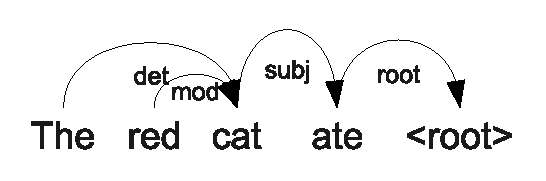
\includegraphics[scale=0.5]{dpm-example-ref.eps} & 
    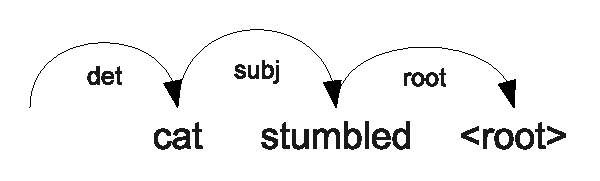
\includegraphics[scale=0.5]{dpm-example-hyp.eps}\\
    \textbf{$dlh$ list} &
    \begin{tabular}{@{$\langle$}c@{,~}c@{,~}c@{$\rangle$}}
      the & \arclabel{\texttt{det}}  &  cat \\
      red & \arclabel{\texttt{mod}}  &  cat \\
      cat & \arclabel{\texttt{subj}} &  ate \\
      ate & \arclabel{\texttt{root}} &  $<$root$>$ \\
    \end{tabular} & 
    \begin{tabular}{@{$\langle$}c@{,~}c@{,~}c@{$\rangle$}}
      the &      \arclabel{\texttt{det}}  &  cat \\
      cat &      \arclabel{\texttt{subj}} &  stumbled \\
      stumbled & \arclabel{\texttt{root}} &  $<$root$>$ \\
    \end{tabular}\\
  \end{tabular}\\
  Precision$_{dlh}$ is $\frac{1}{3}$ and Recall$_{dlh}$ is
  $\frac{1}{4}$: thus $F[dlh] = \frac{2}{7}$
  \caption{Example hypothesis and reference dependency trees and the
    $dlh$ decomposition of each.}
  \label{fig:decompexample}
\end{figure}
illustrates the \emph{dependency-link-head} decomposition of a toy
dependency tree into a list of $\langle d, l, h \rangle$ tuples.  Some
members of the DPM family may apply more than one decomposition; other
good examples are the $dl$ decomposition, which generates a bag of
dependent word with outbound links, and the $lh$ decomposition, which
generates a bag of inbound link labels, with the head word for each
included. 
\begin{figure}
  \centering
    \begin{tabular}{cc}
    $dl$ & $lh$ \\
    \hline
    \begin{tabular}{@{$\langle$}c@{,~}c@{$\rangle$}}
      the & \arclabel{\texttt{det}}  \\
      cat & \arclabel{\texttt{subj}} \\
      stumbled & \arclabel{\texttt{root}} \\
    \end{tabular} &
    \begin{tabular}{@{$\langle$}c@{,~}c@{$\rangle$}}
      \arclabel{\texttt{det} } &  cat \\
      \arclabel{\texttt{subj}} &  stumbled \\
      \arclabel{\texttt{root}} &  $<$root$>$ \\
    \end{tabular}\\
  \end{tabular}
  \caption{The $dl$ and $lh$ decompositions of the hypothesis tree in
    figure~\ref{fig:decompexample}. The items extracted here
    are individually less restrictive in their ability to match
    against reference tuples. 
%     $\precision{dl} = \frac{2}{3}$,
%     $\recall{dl} = \frac{2}{4}$, $\precision{lh} = \frac{2}{3}$,
%     $\recall{lh} = \frac{2}{4}$, so $F[dl,lh] = \frac{4}{7}$
  }
  \label{fig:decompexample2}
\end{figure}
Figure~\ref{fig:decompexample2} demonstrates the $dl,lh$
decomposition for the hypothesis tree in figure~\ref{fig:decompexample}.

It is worth noting here that the $dlh$ and $lh$ decompositions (but
not the $dl$ decomposition) ``overweight'' the headwords, in that
there are $n$ elements in the resulting bag, but if a word has no
dependents it is found in the resulting bag exactly one time (in the
$dlh$ case) or not at all (in the $lh$ case).  Conversely,
syntactically ``key'' words, that are directly modified by many other
words in the tree, are included multiple times in the decomposition
(once for each inbound link).  We argue that this overcounting is a
virtue; the syntactic structure indicates which words are more
important to translate correctly.

We may not completely trust the parser's best parse.  The parser
itself, if we use a probabilistic parser, can provide an $n$-best
parse list for the translation reference and translation
hypothesis. We use the probability statistics of the list to compute
expected counts for each decomposition. Though this approach yields
partial counts, standard comparisons like precision and recall are
still valid, and using the expectations can help cope with both error
in the parser and ambiguity in the translations (reference and
hypothesis).

When multiple decomposition types are used together, we may combine
these subscores in a variety of ways.  We may compute precision and
recall subscores for each decomposition separately, or, since the
results of each decomposition are of different types entirely, we may
compute them as members of one large bag for an even simpler F score.
These two approaches are equivalent when only one decomposition type
is included.  For simplicity in presentation, we use the following
notation, where $dl$ and $lh$ represent the two kinds of
decompositions described above and $\mu_h$ represents a harmonic mean:
\begin{eqnarray}
  \label{eq:fprmeans}
  F[dl,lh] & = &
  \mu_h \left( \precision{dl \cup lh},
    \recall{dl \cup lh} \right) \\
  \mu_{PR}[dl,lh]  & = & \mu_h \left( \precision{dl},
    \recall{dl}, \precision{lh}, \recall{lh} \right)    
\end{eqnarray}
Dependency-based SParseval and the \textbf{d} approach from
\inlinecite{owczarzak07labelleddepseval} may each be understood as
$F[dlh]$, while the latter's \textbf{d\_var} method may be understood
as something close to $F[dl,lh]$.

Both of the combination methods above ($F[\cdot]$ and
$\mu_{PR}[\cdot]$) are ``naive'' in that they treat each component
score as equivalent to the next.  One further direction to explore
involves tuning (presumably on held-out data) the precision and recall
weights for each decomposition type for a later linear combination.

The possible family of metrics outlined above is quite large. In the
next section, we make explicit the range of these parameters that we
explore in this article.


\section{Experimental paradigm}
\label{sec:paradigm}
% In this section, we describe the details of the implementation and
% experimental variables explored in the experiments presented here.

\subsection{Parse tree implementation}
In principle, the family of DPM measures may be implemented with
any parser that generates a dependency graph (a single labelled arc
for each word, pointing to its head-word). Prior work
\cite{owczarzak07labelleddepseval} on related
measures has used an LFG parser \cite{cahill04lfg} or
an unlabelled dependency tree \cite{liu05syntaxformteval}. 

In this work, we use a state-of-the-art PCFG (the first stage of
\inlinecite{charniak-johnson:2005:ACL}) and context-free head-finding
rules \cite{magerman95headfinding} to generate a 50-best list of
dependency trees for each hypothesis and reference translation.  We
use the parser's default (English-language) Wall Street Journal
training parameters.  Head-finding uses the Charniak parser's rules,
with three modifications: prepositional and complementizer phrases
choose nominal and verbal heads respectively (rather than functional
heads) and auxiliary verbs are modifiers of main verbs (rather than
the converse).

Having constructed the dependency tree, we label the arcs as $d
\stackrel{A/B}{\to} h$, where the arc label $A/B$ between dependent
$d$ and its head $h$ is composed of $A$ (the lowest constituent-label
headed by $h$ and dominating $d$) and $B$ (the highest constituent
label headed by $d$).
\begin{figure}
  \Tree
  [.\headlabel{S}{stumbled}
    [.\headlabel{NP}{cat}
      [.\headlabel{DT}{the} the ]
      [.\headlabel{NN}{cat} cat ]
    ]
    [.\headlabel{VP}{stumbled} 
      [.\headlabel{VBD}{stumbled} stumbled ]
    ]
  ]
  \\
  \begin{center}
    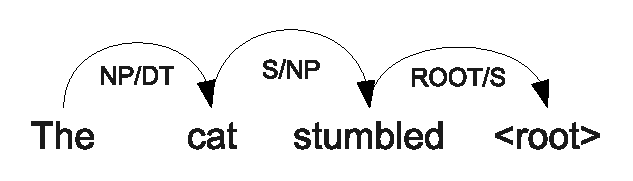
\includegraphics[scale=0.6]{dpm-example-depextract.eps}
  \end{center}
  \caption{An example constituent tree (heads of each constituent are
    listed small below the label) and the labelled dependency tree
    derived from it using the strategy described in
    section~\ref{sec:paradigm}.}
  \label{fig:depextract}
\end{figure}
For example, in figure~\ref{fig:depextract}, the S node is the lowest
node headed by \emph{stumbled} that dominates \emph{cat}, and the NP
node is the highest constituent label headed by \emph{cat}, so the arc
between \emph{cat} and \emph{stumbled} is labelled \arclabel{S/NP}.
%
This strategy is very similar to one adopted in the reference
implementation of labelled-dependency \textsc{SParseval}, and may be
considered as an approximation of the rich semantics generated by LFG
parsers \cite{cahill04lfg} or another heavily knowledge-engineered
parser, but with much less knowledge-engineering required.

The $A/B$ labels are not as descriptive as the LFG semantics, but they
have a similar resolution, e.g.\ the $\stackrel{S/NP}{\to}$ arc label
usually represents a subject dependent of a sentential verb.

\subsection{Dimensions of metric family}
In the experiments presented later in this article, we explore the
space of metrics outlined above along multiple dimensions:
\begin{description}
\item[Decompositions.] We consider syntactic decompositions of the
  following types:
  \begin{description}
  \item[dlh] $\left\langle \textrm{Dependent}, \textrm{arc Label},
      \textrm{Head}\right\rangle$ Here, every tuple includes two words
    and the dependency-label between them.
  \item[dl] $\left\langle \textrm{Dependent}, \textrm{arc Label}
      \right\rangle$ The tuple is the word plus the label of the arc
      linking it to its head; this decomposition marks how the word
      fits into its syntactic context (what it modifies).
    \item[lh] $\left\langle \textrm{arc Label}, \textrm{Head}
      \right\rangle$ Each tuple here is the dependency relation plus
      the word being modified; this decomposition implicitly marks how
      key the word is to the sentence.
    \item[dh] $\left\langle \textrm{Dependent}, \textrm{Head}
      \right\rangle$ Here, drops the arc-label. This decomposition
      ignores the syntactic-role information implied in the arc labels.
    \item[1g,2g] These decompositions are syntactically-null.  They
      simply include each 1-gram (or 2-gram) without any syntactic
      labeling at all.  They are thus simple measures of unigram
      (bigram) precision and recall.
  \end{description}
\item[Size of $n$-best list.] Although the parser can generate
  considerably more, we consider $n$-best lists of size 1 and of size
  50.
\item[Confidence of $n$-best hypotheses.] An expectation requires a
  probability distribution over the $n$-best list, and we consider
  three options: uniform, the parser probabilities, and a flattened
  version of the parser probabilities such that $\tilde{p}(x) =
  \frac{p(x)^\gamma}{\sum_ip(i)^\gamma}$ (where $\gamma$ is a free
  parameter) to account for the fact that the parser tends to be
  over-confident.  In all cases, the probabilities are normalized to
  sum to one over the the $n$-best list, where the maximum $n$ in this
  work is 50.  The uniform distribution ($\gamma = 0$) is intended to
  be equivalent to the \cite{owczarzak07labelleddepseval}
  \textbf{d\_50} and \textbf{d\_50\_var} measures.\footnote{Since
    \inlinecite{owczarzak07labelleddepseval} report no use of parse
    weights, \textbf{d\_50} and \textbf{d\_50\_var} may be using a sum
    of counts over the 50-best list rather than expected-counts over a
    uniform distribution. These two approaches are equivalent --- so
    long as the $n$-best list is always the same length for hypothesis
    and reference.  In our implementation, the $n$-best list does not
    always reach 50 candidate parses on short sentences, so the
    expectation matches our intent better than a sum of counts over
    the $n$-best.}
\item[Score combination.] We consider three possible methods for
  combining scores across decompositions, as suggested in
  section~\ref{sec:approach}:
  \begin{description}
  \item[$F\lbrack\cdot\rbrack$] treats each decomposition as
    contributing $n$ more items to the bag of tokens extracted from
    the tree, and then computes a global $F$ score.
  \item[$\mu_{PR}\lbrack\cdot\rbrack$] constructs a precision and
    recall score from each decomposition, and then does an
    evenly-weighted harmonic mean of all the component precision and
    recall scores.
  \item Tuned, like the previous combination, calculates precision and
    recall separately for each decomposition, but performs a linear
    weighted combination of the resulting precision and recall scores.
    For this tuning, we note that TERp \cite{snover09terp} provides a
    tuneable system over a small number of parameters (they include,
    among others, separate cost for insertions, deletions,
    substitutions and synonyms) and an optimization algorithm that
    assigns weights to each parameter. We use the various
    decompositions' precision and recall as new parameters to the TERp
    optimizer.
  \end{description}
\end{description}

\subsection{Reference evaluation measures over parallel translations}

For some of the experiments presented here (sections~\ref{sec:hter1}
and~\ref{sec:hter2}), we have multiple translations of the same source
segment, each from a different translation engine and each with its
own HTER score.  For these translations, reporting correlations of
metric $m$ with absolute HTER scores can conflate $m$'s power in
identifying which of two candidate translations is better with $m$'s
(and HTER's) ability to distinguish which source segments are more
difficult to translate.

To avoid this conflation, on the HTER corpora we report correlations
on $\bar{\mu}(m)$ and $\bar{\mu}(\textrm{HTER})$ (rather than measure
$m$ and HTER), where $\bar{\mu}$ represents mean-removal:
\begin{equation}
  \label{eq:meansub}
  \bar{\mu}(m(t_i)) = m(t_i) - \sum_{j=1}^I\frac{m(t_j)}{I}
\end{equation}
Mean-removal lowers the correlation $r$ values reported but ensures
that the reported correlations are among differences in the
translations rather than among differences in the underlying segments.
\footnote{ Previous work \cite{kahn08metricsmatr} reported HTER
  correlations against pairwise differences among translation segments
  derived from the same source segment. The results are similar to
  those reported here. However, we believe that pairwise differences
  introduce problems with the independence assumptions in the
  Pearson's $r$ tests, and we use mean-removal throughout this work
  instead.}

%% MO: Okay, but a little hard to figure out.
When reporting HTER correlations per-sentence, we use length-weighted
correlation, since unweighted correlations effectively put too much
emphasis on short sentences.  We do not weight for length for the
per-document correlations in section~\ref{sec:hter1}, because we
assume documents to be equally important (regardless of length).

\section{Correlation with human judgments of fluency \& adequacy}
\label{sec:faexpts}

To explore members of the DPM metric family, we explore the
correlations of various configurations against a corpus of human
judgments of fluency and adequacy.

% TO DO: more to say here?

\subsection{Corpus}

For these experiments, we use LDC Multiple Translation Chinese corpus
parts 2~\cite{LDC03MTC2} and 4~\cite{LDC06MTC4}.  These corpora
include multiple human judgments of fluency and adequacy for each
sentence, with each judgment using a different human judge and a
different reference translation.  For a rough\footnote{Our segment
  count differs from \inlinecite{owczarzak07labelleddepseval}, who
  report 16,800 segments over the same corpus. We find baseline
  correlations (BLEU$_4$ and TER) lower than those reported there as
  well, so the results presented here are not directly comparable with
  that paper, though we demonstrate similar gains over those baselines
  in essentially the same
  corpus. % (section~\ref{sec:facorr:newdeps}).}
} comparison with \inlinecite{owczarzak07labelleddepseval}, we treat
each judgment as a separate segment.
%
This treatment of this corpus yields 16,815 tuples of
$\langle$hypothesis, reference, fluency, adequacy$\rangle$.  In these
experiments, we extend this tuple with automatic scores derived from
$\langle$hypothesis, reference$\rangle$ and examine the
correlations\footnote{The independence of each of these segments is
  questionable, since the same hypothesis translations are used in
  multiple items, but for the sake of methodological comparison with
  prior work, this strategy is preserved.}  between those automatic
scores and the arithmetic mean of the fluency and adequacy measures.

\subsection{Exploring decompositions}
We begin by comparing some of the simplest DPM measures to baseline
measures case-sensitive BLEU (4-grams, with add-one smoothing) and
TER.  For these first experiments, we consider only the 1-best parse
($n=1$).
\begin{table}
  \caption{Comparing $dl,lh$ to $dlh$ and baselines.}
  \label{tab:facorr:subgraphs}
  \begin{tabular*}{2.5in}{lr}
    \hline
    metric  &    \multicolumn{1}{c}{$r$} \\
    \hline
    $F[dl,lh]$ &   0.226 \\
    % # +1 smoothing
    BLEU$_4$ &   0.218 \\
    $F[dlh]$ &     0.185 \\
    TER &      -0.173 \\
    \hline
  \end{tabular*}
\end{table}
In table~\ref{tab:facorr:subgraphs} we see that using the
partial-label $dl,lh$ decomposition has a better correlation with the
fluency/adequacy scores than TER or BLEU$_4$.  These results confirm,
with a PCFG, what \inlinecite{owczarzak07labelleddepseval} found with
an LFG parser: that partial-dependency matches are better correlated
with human judgments than full-dependency links.

In table~\ref{tab:facorr:combinations}, we compare among several other
members of the DPM family. 
 \begin{table}
  \begin{tabular*}{2.5in}{lr}
    \hline
    metric  &    \multicolumn{1}{c}{$r$} \\
    \hline
    $F[1g,2g,dl,lh]$      &  0.237 \\
    $\mu_{PR}[1g,2g,dl,lh]$ &  0.217 \\
    \rlcline{1-1} \rlcline{2-2}
    $F[1g,2g]$            & 0.227 \\
    $F[1g,dl,dlh]$        & 0.227 \\
    \rlcline{1-1} \rlcline{2-2}
    $F[dl,lh]$            &  0.226 \\
    $\mu_{PR}[dl,lh]$      &  0.208 \\
    \hline
  \end{tabular*}
  \caption{Comparing combination methods $F[\cdot]$ and
    $\mu_{PR}[\cdot]$, and comparing the $1g,2g,dl,lh$ decomposition
    with the $dl,lh$ decomposition and other decompositions.}
  \label{tab:facorr:combinations}
\end{table}
Here, we find that combining the decompositions naively in $F[\cdot]$
(before computing precision and recall) has a better $r$ than the
harmonic mean of precision and recall subscores in $\mu_{PR}[\cdot]$.
We also see that we can combine the benefits of string-local $n$-grams
($F[1g,2g]$) with the benefits of dependency information ($F[dl,lh]$)
for a further improved correlation with human judgment, with the best
correlation in $F[1g,2g,dl,lh]$. Including progressively larger chunks
of the dependency graph (as in $F[1g,dl,dlh]$, which is inspired by
the BLEU$_k$ idea of progressively larger $n$-grams) does not seem to
be an improvement over $F[dl,lh]$.

% (too many chances for zeroes?)

\subsection{Exploring parse expectations}

To explore the effect of extracting parse feature-counts from a forest
instead of a single tree, we present in
table~\ref{tab:facorr:multiparse} several variants, with $n=1$ and
with $n=50$.
 \begin{table}
  \begin{tabular*}{2.5in}{lrr}
    \hline
    metric  & \multicolumn{1}{c}{$n$} &  \multicolumn{1}{c}{$r$} \\
    \hline
    $F[1g,2g,dl,lh]$      & 50 &  0.239 \\
    $F[1g,2g,dl,lh]$      &  1 &  0.237 \\
    \rlcline{1-2}\rlcline{3-3}
    $F[1g,dl,lh]$            &  50 & 0.237 \\
    $F[1g, dl,lh]$            &  1 & 0.234 \\
    \rlcline{1-2}\rlcline{3-3}
    $F[dl,lh]$            &  50 & 0.234 \\
    $F[dl,lh]$            &  1 & 0.226 \\
    \hline
  \end{tabular*}
  \caption{Comparing $n=1$ to $n=50$ for several variants of the DPM measure.}
  \label{tab:facorr:multiparse}
\end{table}
For the $n=50$ cases, we set $\gamma=0$ to assign uniform
probabilities to the parse forest, to compare as closely as possible
to \inlinecite{owczarzak07labelleddepseval}, which includes a
\textbf{d\_var\_50} measure with 50-best parses, with ranks but no
weights.  While not all of these differences are significant, the
trend is universally that the correlation $r$ improves as the number
of parses ($n$) is increased.  Tuning experiments find that increasing
$\gamma$ to 0.25 can increase the $r$ reported here for
$F[1g,2g,dl,lh]$ marginally (but insignificantly).

\subsection{Summary}

In this section, we have presented experiments exploring a number of
variants of the DPM metric against an average fluency/adequacy
judgment. The experiments suggest a best-case variant, where we set:
\begin{displaymath}
  EDPM = F[1g,2g,dl,lh], n=50, \gamma=0.25
\end{displaymath}
in which we choose a $1g,2g,dl,lh$ sub-graph decomposition based on
the improvements from better sub-graphs
(table~\ref{tab:facorr:subgraphs}), multiple parses ($n=50$) based on
table~\ref{tab:facorr:multiparse}, and $\gamma=0.25$.
%, hinted at by table~\ref{tab:facorr:parseweight}.  
We use these EDPM parameter-settings in the experiments exploring
document-level correlations with HTER (section~\ref{sec:hter1}).


\section{Correlating EDPM with HTER}
\label{sec:hter1}
In this section, we move from an exploration of the space of possible
DPM metrics to a single chosen DPM-derived metric (EDPM).  Here, we
compare EDPM to other metrics in correlation with document-level and
segment-level HTER performance.

\subsection{HTER corpus}

The GALE 2.5 translation corpus is made up of system translations into
English from three sites.
%
The three sites all use system combination to integrate results from
multiple systems, some of which are phrase-based and some which may
use syntax on either the source or target side. No system provided
system-generated parses.
%
The corpus being translated comes from Arabic and Chinese in four
genres: \texttt{bc} (broadcast conversation), \texttt{bn} (broadcast
news), \texttt{nw} (newswire), and \texttt{wb} (web text), with corpus
sizes shown in table~\ref{tab:galestats}.
\begin{table}
  \begin{tabular}{r|rr|rr|rr}
    \hline
     & \multicolumn{2}{c|}{Arabic} & \multicolumn{2}{c|}{Chinese}
     & \multicolumn{2}{c}{Total}\\
     & doc & sent & doc & sent & doc   & sent\\
     \hline
     \texttt{bc}    & 59  & 750 & 56 & 1061 & 115 & 1811\\
     \texttt{bn}    & 63  & 666 & 63 & 620  & 126 & 1286\\
     \texttt{nw}    & 68  & 494 & 70 & 440  & 138 & 934 \\
     \texttt{wb}    & 69  & 683 & 68 & 588  & 137 & 1271\\
     \hline
     Total & 259 & 2593& 257& 2709 & 516 & 5302\\
     \hline
  \end{tabular}
  \caption{Corpus statistics for the GALE 2.5 translation
    corpus.}
  \label{tab:galestats}
\end{table}
The corpus includes one English reference translation $r_i$
\cite{gale08phase2_5references} for each sentence $i$ and a system
translation $t_{i,z}$ for each of the three systems $z$. Additionally,
each of the system translations of each segment $i$ has a
corresponding human-targeted reference aligned at the sentence level,
so we have available the HTER score of each segment HTER$(t_{i,z})$ at
both the sentence and document level.

As discussed in section~\ref{sec:paradigm}, we report correlations
here between $\bar{\mu}(m)$ and $\bar{\mu}(\textrm{HTER})$, rather
than $m$ and HTER directly, to abstract away from variations in the
underlying documents.

In table~\ref{tab:hterperdoc}, we show per-document Pearson's $r$
between $\bar{\mu}$EDPM and $\bar{\mu}$HTER, as well as two other
baselines: $\bar{\mu}$TER and $\bar{\mu}$BLEU$_4$.
\begin{subtable}
  \begin{table}
    \begin{tabular}{r|rrrr|rr|r}
      \hline
      $r$ vs. $\bar{\mu}$HTER & \multicolumn{1}{c}{\texttt{bc}}
      & \multicolumn{1}{c}{\texttt{bn}} &
      \multicolumn{1}{c}{\texttt{nw}} & \multicolumn{1}{c}{\texttt{wb}}
      & \multicolumn{1}{|c}{all Arabic} & \multicolumn{1}{c|}{all Chinese}
      & \multicolumn{1}{c}{all} \\
      \hline
      $\bar{\mu}$TER
      &  0.59 &  \textbf{0.35} &  \textbf{0.47}&  \textit{0.17}
      & \textbf{0.54} & \textbf{0.32} &  0.44\\
      $\bar{\mu}$BLEU
      & -0.42 & \textbf{-0.32} & \textbf{-0.46}&  \textbf{-0.27}
      & -0.42  &  \textbf{-0.33} & -0.37 \\
      $\bar{\mu}$EDPM
      & \textbf{-0.69} & \textbf{-0.39} & \textbf{-0.47} &
      \textbf{-0.27}
      & \textbf{-0.60} & \textbf{-0.39} & \textbf{-0.50} \\
      \hline
    \end{tabular}
    \caption{Per-document correlations of $\bar{\mu}$EDPM and others to
      $\bar{\mu}$HTER, by genre and by source language. Bold numbers are
      within 95\% significance of the best per column; italics indicate
      that the sign of the $r$ value has less than 95\% confidence.}
    \label{tab:hterperdoc}
  \end{table}
  \begin{table}
    \begin{tabular}{r|rrrr|rr|r}
      \hline
      $r$ vs. $\bar{\mu}$HTER & \multicolumn{1}{c}{\texttt{bc}}
      & \multicolumn{1}{c}{\texttt{bn}} &
      \multicolumn{1}{c}{\texttt{nw}} & \multicolumn{1}{c}{\texttt{wb}}
      & \multicolumn{1}{|c}{all Arabic} & \multicolumn{1}{c|}{all Chinese}
      & \multicolumn{1}{c}{all} \\
      \hline
      $\bar{\mu}$TER
      &  \textbf{0.44} &  \textbf{0.29} &  \textbf{0.33}&  0.25
      & \textbf{0.44} & 0.25  &  \textbf{0.36}\\
      $\bar{\mu}$BLEU
      & -0.31 & -0.24  & -0.29 &  -0.25
      & -0.31  &  -0.24  & -0.28 \\
      $\bar{\mu}$EDPM
      & \textbf{-0.46} & \textbf{-0.31} & \textbf{-0.34} &
      \textbf{-0.30}
      & \textbf{-0.44} & \textbf{-0.30} & \textbf{-0.37} \\
      \hline
    \end{tabular}
    \caption{Per-sentence, length-weighted correlations of
      $\bar{\mu}$EDPM and others to $\bar{\mu}$HTER, by genre and by
      source language.}
    \label{tab:hterpersent}
  \end{table}
\end{subtable}
We see that the EDPM has the highest correlation in each of the
subcorpora created by dividing by genre or by source language, as well
as the corpus as a whole.  Not every difference is above 95\%
confidence, but the trend is the same across all of the
subcorpora. EDPM's strengths, relative to the other measures, are
particularly clear in the unstructured domains (\texttt{wb} and
\texttt{bc}).

%% MO: I still think this is a bit weird given that what you are
%% adding is structure. If time, you might want to look at some
%% example sentences
Table~\ref{tab:hterpersent} presents per-sentence correlations,
weighted by sentence length.  Though many of the $r$ values are
smaller magnitude in this correlation, EDPM again has the largest
correlation in each category.  TER, however, does quite well with
length-weighted sentence correlation, with $r$ values within 95\%
confidence of EDPM scores on nearly every breakdown.

\section{Weight-tuning to combine syntax and other knowledge sources}
\label{sec:hter2}

In the previous section, we observed that TER and EDPM each perform
better than BLEU when considering mean-removed length-weighted
correlations with HTER.  We observe that TER's basic operations
(insertions, deletions, shifts and substitutions) are fundamentally
different from those of EDPM, which is an $F$-style overlap measure
and is seeking to make explicit comparison based on an inferred
syntactic structure.  These two different approaches (word-level and
syntactic features) are complementary, and we seek in this section to
explore mechanisms for combining them.

As discussed in section~\ref{sec:intro}, the TER Plus (TERp) research
tools \cite{snover09terp} provide an optimizer for weighting multiple
simple subscores, including selecting weights for the TER basic
operations. TERp's feature list extends TER to additionally include
synonym tables and an empirically-derived paraphrase table.

%% MO: important to describe basic model before listing features.
TO DO: TERp optimizer [Matt, a brief description here]

In the experiments presented in this section, we extend this feature
list by including the syntactic overlap features, and we use the TERp
optimizer tools to tune the relative weight of each feature.

\subsection{Features}

We train a model using features from one or more of the following
sets:
\begin{description}
\item[E]: the fully syntactic features from the DPM family.
  Specifically, this feature set includes precision and recall scores
  for the $dl$, $lh$, $dlh$, and $dh$ decompositions of the syntactic
  structure, using $n=50$ and $\gamma=0.25$.  The \textbf{E} set
  includes 8 features.
\item[N]: the non-syntactic features from the DPM family;
  specifically, precision and recall for $1g$ and $2g$ decompositions.
  The \textbf{N} set includes 4 features.
\item[T]: the features from basic TERp, which include a separate cost
  for each of insertions, deletions, substitutions, shifts, and
  synonym-alignment. The \textbf{T} set includes 7 features.
  % MO  (to Matt): is this basic TER or basic TERp?
  % TO DO: what are the other two?
\item[P]: features from the automatically-derived TERp paraphrase
  table (4 features) % TO DO: Matt, what are these
\item[B]: two ``length penalties'' one is assigned the count of
  hypothesis words beyond the count of reference words, and one
  assigned the count of reference words beyond the count of hypothesis
  wordsbrevity/prolixity (2 features: one for longer-than-ref, one for
  shorter-than-ref).
  % MO: out of curiosity, why do you need 2 features?
  We assign two features here to let the system separately penalize
  ``too short'' translations and ``too long''.
\end{description}

\subsection{Corpus}

For these tuning experiments we use the same GALE 2.5 documents and
sentences from the previous section.  Since this approach requires
tuning, we assign documents randomly into two groups, such that each
group has the same document distribution across source-language and
genre.
%
These two corpus halves are used in two-fold cross-validation, testing
on one and training on the other.  We tune on (and report correlation
with) length-weighted per-sentence correlation with HTER, using
mean-removed scores as before.

% tuning target: weighted correlation with mean-removed segment HTER

% [we use weighted correlation to avoid emphasis on short segments
% (which hurts document-level and system-level utility) ]
In figure~\ref{fig:tuneresults}, we plot the Pearson's $r$ (with 95\%
confidence interval) for the results on the two test sets (each
trained on one and tested on the other).
\begin{figure}
  \centerline{{one figure}\qquad{}{two figure}}
  \caption{Figure with two tune-set plots will go here.}
  \label{fig:tuneresults}
\end{figure}


% MO suggestions:

%% do n-fold with >2 N -- better robustness to variation?

%% look at variation in weights on 2-fold case   
\begin{verbatim}
   == Tuned For Weighted Mean Removed Pearson
     - Examining WGT_MEAN_RM_SEG_PEAR ==
            Average
      Cond   Test  
     ---------------
      ETPB   0.4096
      ETP    0.4038
      TPB    0.4010
      TP     0.3946  > 0.416
      TPNB   0.3940
      TPN    0.3891
      ETB    0.3871
      ET     0.3827  > 0.404
      TB     0.3815  > 0.403
      ETNB   0.3814
      ETN    0.3804
      T      0.3758  > 0.398
      TNB    0.3708
      TN     0.3680  > 0.390
      TER    0.353   > 0.375
      E      0.3287  > 0.352
      EB     0.3267
      ENB    0.3149
      NB     0.3058  > 0.329
      EN     0.2973
      N      0.2636
      BLEU   0.244
      B      0.1638
\end{verbatim}
(maybe don't report all these numbers!)

TO DO: discuss this as a trend, despite lack of significance? plot charts?
  
point: E+T $>$ T, E+TB $>$ TB, E+TP $>$ TP; information is available
in syntax that is not captured in the other measures.

point: syntax is *not* just an expensive way to get at n-grams;
N-grams are not the same -- TP $>$ TP+N, but TP $<$ TP+E

question: this is kind of like the $\mu_{PR}[\cdot]$ --- seems like it
also doesn't work so well. compare to EDPM as-is

talk about why EN is $<$ EDPM (is it?)

\section{Conclusion}
\label{sec:conclusion}
In this research, we explore dependency pair match (DPM) a family of
syntactically-oriented measures.  Through a corpus of human judgments,
we settle on EDPM, a member of that family with promising predictive
power.  We find that EDPM is superior to BLEU and TER in terms of
correlation with human judgments and as a per-document and
per-sentence predictor of HTER (using mean-subtraction to account for
underlying document- and segment-level difficulty).
% TO DO:  add something here regarding summary of tuning?

Several areas of future work are open to us. One obstacle to using
this method widely is the computational expense of the system. Parsing
is many times more computationally costly than word-based measures
such as BLEU or TER.  Using these syntactic techniques may be possible
as a late-pass evaluation, to identify how candidate translation
systems are performing overall.  Alternatively, the various
tree-decompositions of the DPM family could be used as system
diagnostics, by looking at relative quality of these component scores
compared to those of an alternative candidate system.

Another interesting research area is in the quality of the parser.  In
this work, we demonstrated that the
\inlinecite{charniak-johnson:2005:ACL} PCFG parser could serve in
place of the LFG parser used in
\inlinecite{owczarzak07labelleddepseval}. PCFG parsers, however, are
fairly easily adaptable to another domain. One interesting research
direction explores the intersection of genre (and genre-mismatch),
parser quality, and prediction of human performance.
% Another
% consideration is the speed of the parser: parse time currently takes
% much, much longer than BLEU, TER, or other word-based measures. 
We are interested in the trade-offs --- if any --- among parse
quality, speed, and predictive power as a translation metric.  One
possibility, for example, is to store packed forests
\cite{huang08packedforests} rather than generating an $n$-best list
only to sum across it again in calculating the expectation.

TO DO: parting words

% \appendix
% [don't think we want an appendix]

\acknowledgements

{\small This material is based upon work supported by the National
  Science Foundation under Grant No. 0741585 and the Defense Advanced
  Research Projects Agency under Contract Nos. HR0011-06-C-0022 and
  HR0011-06-C-0023.

% Re: DARPA contract numbers
% -0022 is Matt's [Agile] grant.
% -0023 is Mari & Jeremy's [Nightingale] grant

  Any opinions, findings, and conclusions or recommendations expressed
  in this material are those of the author(s) and do not necessarily
  reflect the views of the National Science Foundation or the Defense
  Advanced Research Projects Agency.  }

% The endnotes section will be placed here.  But I don't think we have any

% \theendnotes

\bibliographystyle{klunamed}
\bibliography{mtjournal}

\end{article}
\end{document}
